\documentclass[tikz,border=8pt]{standalone}
% Shared look for every TikZ diagram. Load with \input{../../tools/tikz-style.tex}
\usepackage[T1]{fontenc}
\usepackage{lmodern}
\renewcommand{\sfdefault}{lmr}  % diagrams use the same serif as the text
\usetikzlibrary{arrows.meta, positioning, shapes.geometric, calc, fit, backgrounds}
\definecolor{cblue}{HTML}{4C78A8}
\definecolor{corange}{HTML}{F58518}
\definecolor{cgreen}{HTML}{54A24B}
\definecolor{cred}{HTML}{E45756}
\definecolor{cpurple}{HTML}{B279A2}
\definecolor{cgrey}{HTML}{6B6B6B}
\tikzset{
  every picture/.style={font=\sffamily, line width=1.2pt},
  box/.style={draw=#1, fill=#1!12, rounded corners=4pt, align=center, inner sep=7pt, minimum height=1.1cm},
  box/.default=cgrey,
  arrow/.style={-{Stealth[length=3mm]}, draw=cgrey, line width=1.4pt},
  title/.style={font=\sffamily\bfseries\Large},
  note/.style={font=\sffamily\small, text=cgrey, align=center},
}
\AtBeginDocument{\hyphenpenalty=10000 \exhyphenpenalty=10000}

\begin{document}
\begin{tikzpicture}[s/.style={box=cblue, minimum width=2.5cm, font=\sffamily\normalsize, align=center},
                    c/.style={font=\ttfamily\small, text=cgrey, align=center}]
  \node (img) at (0,0) {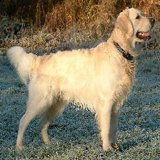
\includegraphics[width=2.4cm]{../data/photos/00.jpg}};
  \node[c, below=1pt of img] {dog.jpg};
  \node[s] (r) at (3.6,0) {resize\\$224\times224\times3$};
  \node[c, below=3pt of r] {load\_img};
  \node[s] (b) at (7.0,0) {batch of one\\$1\times224\times224\times3$};
  \node[c, below=3pt of b] {expand\_dims};
  \node[s] (p) at (10.4,0) {RGB$\to$BGR,\\subtract channel\\means};
  \node[c, below=3pt of p] {preprocess\_input};
  \node[box=corange, minimum width=2.5cm, align=center] (m) at (13.8,0) {\textbf{ResNet50}\\25,636,712\\parameters};
  \node[c, below=3pt of m] {model.predict};
  \node[box=cgreen, align=left, font=\sffamily\normalsize] (o) at (17.6,0)
    {1,000 probabilities\\[2pt]golden retriever 0.92\\Labrador retriever 0.04\\kuvasz 0.03};
  \node[c, below=3pt of o] {decode\_predictions};
  \foreach \x/\y in {img/r, r/b, b/p, p/m, m/o} \draw[arrow] (\x) -- (\y);
\end{tikzpicture}
\end{document}
